\chapter{Strumenti utilizzati}
\label{cap:strumenti-utilizzati}

\intro{Il seguente capitolo ha la funzione di introdurre tutti gli strumenti utilizzati come supporto alle attività di sviluppo dell'applicativo, tra cui: ambiente di lavoro, framework, linguaggi, librerie a supporto della codifica e IDE. Tutte le  tecnologie elencate rappresentano vincolo di sviluppo del progetto.}

\setlength{\parskip}{3ex}

\section{Ambiente di lavoro}
CWBI ha a disposizione circa 30 macchine fisiche con sistema operativo Debian, ciascuna delle quali viene utilizzata come supporto per delle macchine virtuali in ambiente Windows 7. Il lavoro quotidiano viene svolto in ambiente virtuale e non fisico; per la connessione alla propria macchina virtuale viene utilizzato il software \textit{VMware Workstation}. Il vantaggio nell'utilizzare macchine virtuali sta nel fatto che tutti i dipendenti presentano la medesima configurazione dell'ambiente di sviluppo e, essendo il lavoro in azienda molto collaborativo, al presentarsi di un problema o di un dubbio sul "cosa fare" i colleghi possono connettersi alla macchina virtuale dove si è presentato il problema per aiutare e velocizzare lo scambio di idee sul come fare.

\pagebreak

\section{Framework}
Nella seguente sezione sono riportati i {\hyperref[para:framework-definition]{framework}}\glsfirstoccur \; utilizzati nelle attività di sviluppo del progetto commissionato. 

\subsection{Spring (core)}

\begin{figure}[!h]
	\centering
	
\includegraphics[width=4cm]{../images/Spring-logo.png}
	\caption{Logo di Spring}
\end{figure}

\noindent {\hyperref[para:spring-site]{Spring}}\ap{{[b]}} è un framework open source nato per lo sviluppo di applicazioni Java EE. Una delle sue maggiori peculiarità risiede nell'essere \textbf{modulare}, il che consente di utilizzare anche solo una parte delle funzionalità che il framework mette a disposizione. Altro punto di forza è la facile integrazione con altri framework esistenti, come: Hibernate, Apache Struts, ecc. 

\setlength{\parskip}{3ex}

\noindent Per lo sviluppo back-end viene utilizzato solamente il  \textit{core container} offerto dal framework:

\begin{figure}[!h]
	\centering
	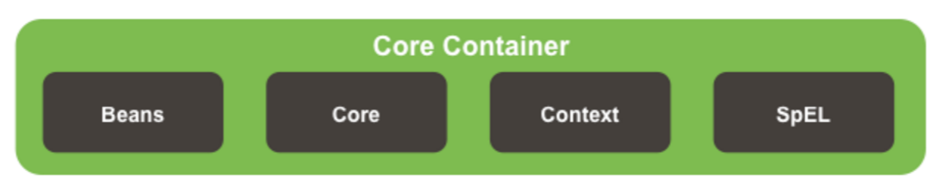
\includegraphics[width=10cm]{../images/Spring-core.png}
	\caption{Spring - core container}
\end{figure}

\begin{enumerate}
\item il modulo bean fornisce le classi factory per l’istanziazione dei bean;
\item il modulo core è la componente fondamentale del framework ed implementa la Dependency Injection;
\item il modulo context fornisce l’accesso a tutti i bean definiti in funzione dei relativi contesti;
\item il modulo SpEL fornisce un expression language per la manipolazione dei bean a runtime.
\end{enumerate}

\pagebreak

\subsection{Hibernate}

\begin{figure}[!h]
	\centering
	
\includegraphics[width=6cm]{../images/Hibernate-logo.png}
	\caption{Logo di Hibernate}
\end{figure}

\noindent Hibernate è un framework open source che permette di  rendere persistenti i dati dall'ambiente Java al database mappando gli oggetti in apposite tabelle di un database relazionale.

\setlength{\parskip}{3ex}

\noindent {\hyperref[para:hibernate-site]{Hibernate}}\ap{{[b]}} gestisce inoltre l'accesso e la manipolazione dei dati stessi generando automaticamente le query in linguaggio SQL; questo agevola il lavoro dello sviluppatore, che non si deve occupare della scrittura manuale delle query di accesso ai dati del database ma solamente di definire gli oggetti che andranno memorizzati e gestiti nel database.

\setlength{\parskip}{2ex}

\noindent Il vantaggio principale nell'utilizzare Hibernate risiede nel fatto che è il framework stesso a costruire le query e questo rende portabili le applicazioni sui diversi servizi di database esistenti (MySQL, PostgreSQL, MariaDB, ecc.).

\subsection{Bootstrap}

\begin{figure}[!h]
	\centering
	
\includegraphics[width=3cm]{../images/Bootstrap-logo.png}
	\caption{Logo di Bootstrap}
\end{figure}

\noindent {\hyperref[para:bootstrap-site]{Bootstrap}}\ap{{[b]}} è un framework open source per lo sviluppo di interfacce web basato su CSS. Bootstrap mette a disposizione una serie di file CSS contenenti stili e regole applicabili ai vari componenti HTML5.

\setlength{\parskip}{3ex}

\noindent Gli stili che bootstrap propone sono ottimizzati per la visualizzazione smartphone, tablet e desktop. Inoltre, dato che la maggior parte degli accessi ad applicativi web avviene tramite cellulare, il framework mette al primo posto il layout per smartphone.\\
Bootstrap è inoltre compatibile con i browser più moderni.

\pagebreak

\subsection{Apache Struts}

\begin{figure}[!h]
	\centering
	
\includegraphics[width=4cm]{../images/Struts-logo.png}
	\caption{Logo di Apache Struts}
\end{figure}

\noindent {\hyperref[para:struts-site]{Apache Struts}}\ap{{[b]}} è un framework open source Java che aiuta gli sviluppatori a creare applicazioni web flessibili, gestibili e sicure in Java. Il framework è caratterizzato da un architettura MVC che consente di raccogliere le richieste provenienti dalla vista e richiamare attraverso il controller le operazioni del modello necessarie a rendere persistenti i dati nel database. Tale architettura si integra con il framework Spring sopra citato.

\pagebreak

\section{Linguaggi utilizzati}
Nella seguente sezione sono riportati i linguaggi utilizzati nella codifica dell'applicativo commissionato.

\subsection{Java}

\begin{figure}[!h]
	\centering
	
\includegraphics[width=3cm]{../images/Java-logo.png}
	\caption{Logo di Java}
\end{figure}

\noindent Per lo sviluppo dell'applicativo lato back-end si è utilizzato Java, un linguaggio di programmazione orientato agli oggetti. La caratteristica principale di questo linguaggio risiede nel rendere indipendente la scrittura di codice dall'ambiente di esecuzione fisico instanziando un ambiente di esecuzione virtuale del codice noto come JVM.

\subsection{HTML5, CSS3 e JavaScript}

\begin{figure}[!h]
	\centering
	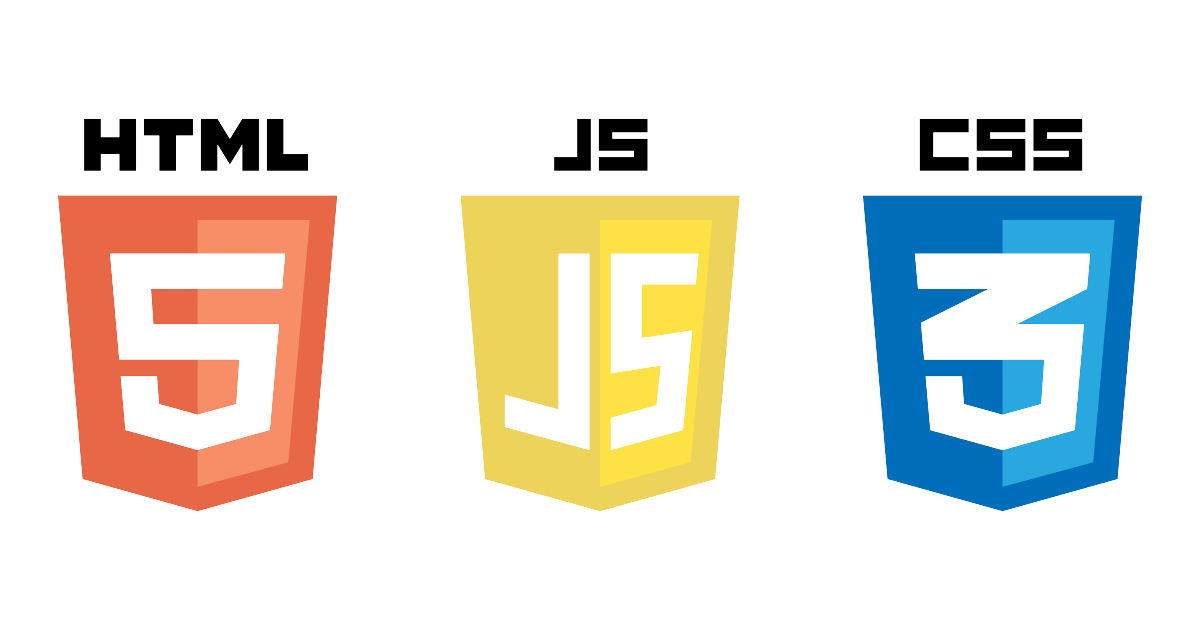
\includegraphics[width=5cm]{../images/HTML5-logo.png}
	\caption{Logo dello stack tecnologico del front-end}
\end{figure}

\noindent Per lo sviluppo dell'applicativo lato front-end si è utilizzato lo stack tecnologico costituito da:
\begin{itemize}
\item HTML5: linguaggio di markup per la creazione di siti web;
\item CSS3: linguaggio utilizzato per definire la formattazione dei documenti HTML attraverso apposite regole di stile;
\item JavaScript: linguaggio di programmazione multi paradigma orientato agli eventi.
\end{itemize}

\pagebreak

\section{Librerie a supporto della codifica}
Nella seguente sezione sono riportate le librerie utilizzate nelle attività di sviluppo del progetto commissionato. 

\subsection{Apache Commons}

\begin{figure}[!h]
	\centering
	
\includegraphics[width=6cm]{../images/Commons-logo.png}
	\caption{Logo di Apache Commons}
\end{figure}

\noindent {\hyperref[para:commons-site]{Apache Commons}}\ap{{[b]}} è una libreria Java molto utilizzata nello sviluppo di applicazioni basate su Java. Questa libreria offre molte classi caratterizzate da diversi metodi che possono essere richiamati dallo sviluppatore semplicemente importando la relativa classe di interesse. Alcune tra le classi offerte sono le seguenti:
\begin{itemize}
\item StringUtils: implementa una serie di operazioni sulle stringhe che completano/estendono quelle offerte dalla classe standard java.lang.String;
\item ArrayUtils: implementa dei metodi che consentono di processare e controllare gli array; 
\item NumberUtils: implementa una serie di metodi a supporto dei tipi numerici offerti da Java.
\end{itemize} 

\subsection{JSTL}
\noindent JavaServer Pages Standard Tag Library (JSTL) è una libreria utilizzata nello sviluppo di applicazioni web Java EE. È un'estensione di Java Server Page (JSP) ed incorpora un insieme di tag HTML definiti tramite file XML e programmati in linguaggio Java. Oltre ai tag standard proposti dalla libreria, JSTL permette allo sviluppatore di definire dei tag custom. 

\setlength{\parskip}{3ex}

\noindent Il vantaggio della creazione di tag risiede nel definire dei comportamenti univoci dello stesso tag in contesti diversi eliminando la necessità di definire funzioni che si ripetono all'interno delle pagine.

\pagebreak

\section{IDE}

\begin{figure}[!h]
	\centering
	
\includegraphics[width=4cm]{../images/Eclipse-logo.png}
	\caption{Logo di Eclipse}
\end{figure}

\noindent Eclipse è un ambiente di sviluppo che supporta diversi linguaggi, tra cui Java. Questo {\hyperref[para:ide-definition]{IDE}}\glsfirstoccur \; è stato utilizzato per lo sviluppo dell'intero progetto.
Tra le diverse funzionalità offerte da questo ambiente troviamo:
\begin{itemize}
\item importare un progetto esistente;
\item creare un nuovo progetto;
\item attività di refactor;
\item attività di debugging.
\end{itemize}